\section{Results}
\label{sec:results}

\subsection{Which settings change the logits}
Table~\ref{tab:kl} is the teacher-forced map: for each model file and each execution-equivalent
setting, the mean KL divergence of the next-token distribution from the reference and the
fraction of positions whose top-1 token is unchanged.

\begin{table}[t]
\centering\scriptsize
\caption{Teacher-forced divergence from the reference configuration on 12 chunks of 512 WikiText
tokens. Each cell is mean KLD / top-1 agreement (\%). ``$=$'' marks a setting that is
indistinguishable from the reference at the tool's storage precision (mean $|$KLD$|$ $\le
10^{-6}$ and 100\% top-1 agreement). UBSIXFOUR Reference: \texttt{alderlake}, 4 threads, micro-batch 512, flash
attention off, repack on.}
\label{tab:kl}
\begin{tabular}{lr}
\toprule
configuration & q06-q4km\\
\midrule
ref-rerun & $=$\\
isa-haswell & $=$\\
isa-ivybridge & 1.2e-2 / 94.1\\
isa-sandybridge & 1.1e-2 / 94.3\\
isa-sse42 & 1.1e-2 / 93.8\\
\bottomrule
\end{tabular}

\end{table}

Two groups appear. Rerunning the reference, changing the thread count, and the
\texttt{haswell} tier are indistinguishable from the reference for every model; so are
micro-batches of 8 and 64. Every other setting differs from the reference for at least one
model, and the differences within a model are of one size: for Q4\_K\_M every differing setting
gives a mean KLD between 0.011 and 0.012 and changes the top-1 token at 5.4 to 6.2\% of
positions, whether the change is the backend tier, micro-batch 1, flash attention or turning
repacking off. The size depends on the weight format, not on which setting caused the
difference: about $10^{-2}$ for Q4\_K\_M, $2.5\times10^{-3}$ for Qwen3 Q4\_0, $1.3\times10^{-3}$
for Q8\_0, Gemma Q4\_0 and Qwen3.5 Q4\_0, and $2\times10^{-6}$ for F16, where only one to three
of 3,072 top-1 tokens change. Section~\ref{sec:mechanism} explains this pattern.

Which settings differ also depends on the format. Turning repacking off changes nothing for
Q8\_0 and F16, which are not repacked on x86, and micro-batch 7 changes only Q4\_K\_M.

\subsection{What the differences do to benchmark answers}
Teacher-forced divergence is a property of the logits; what matters to a benchmark user is
whether answers change. Table~\ref{tab:eval} summarizes the benchmark runs for the primary model
(the full table for all models is Table~\ref{tab:evalfull} in the appendix).

\begin{table}[t]
\centering\small
\caption{Benchmark runs of Qwen3-0.6B Q4\_K\_M against the reference run $R$ (980 items: 600
MMLU, 300 TriviaQA, 80 GSM8K). ``ident.'': items whose tokens and log-probabilities are bitwise
equal to $R$. ``same out'': items whose generated tokens are equal. Flips are over all 980
items, reference right and other wrong / reference wrong and other right. $p$: exact McNemar
test on the flips. The last row compares the two \texttt{server4} runs with each other.}
\label{tab:eval}
\begin{tabular}{lrrrrrrrr}
\toprule
configuration & ident. \% & same out \% & MMLU ans. changed & flips & $p$ & $\Delta$MMLU & $\Delta$TQA & $\Delta$GSM\\
\midrule
ref-rerun & 100.0 & 100.0 & 0 & 0 (0/0) & 1.00 & +0.0 & +0.0 & +0.0\\
sandybridge tier & 0.0 & 79.7 & 41 & 37 (15/22) & 0.32 & +0.5 & +1.0 & +1.3\\
micro-batch 7 & 0.0 & 80.2 & 49 & 47 (23/24) & 1.00 & +0.2 & -0.3 & +1.3\\
prompt cache on & 31.7 & 91.2 & 22 & 23 (14/9) & 0.40 & -0.5 & -0.7 & +0.0\\
server4 (run a) & 11.6 & 85.6 & 21 & 32 (13/19) & 0.38 & +0.3 & +0.7 & +2.5\\
server4 (run b) & 11.5 & 85.0 & 20 & 25 (9/16) & 0.23 & +0.0 & +1.7 & +2.5\\
server4 a vs b & 45.4 & 87.9 & 13 & 17 (8/9) & 1.00 & -0.3 & +1.0 & +0.0\\
\bottomrule
\end{tabular}

\end{table}

A second run of $R$ reproduced all 980 items bit for bit, so the reference is deterministic and
every difference below comes from the one changed setting. Loading the AVX tier
(\texttt{sandybridge}) instead of \texttt{alderlake} left no item bitwise identical: every
first-step log-probability moved (median change of the top token's log-probability 0.10 nats).
One generated output in five differed, 41 of 600 MMLU answers changed and 37 items flipped
between right and wrong (15 one way, 22 the other). Micro-batch 7 did the same (49 MMLU answers
changed, 47 flips). Yet every accuracy moved by at most 1.3 points, and no McNemar test was close
to significance ($p\ge0.32$). The flips cancel because they are not caused by the model getting
better or worse; they are coin tosses on items the model was unsure about.

That is visible in the reference margins (Figure~\ref{fig:margins}, left). Across the five
benchmark settings that differ from $R$, 71 distinct MMLU items changed their answer at least
once. Their median reference margin was 0.28 nats, against 1.65 for all items. Of the 44 items
with a margin under 0.25 nats, 33 changed under at least one setting; of the 424 items with a
margin of at least 1 nat, one did. The largest margin that changed was 1.25 nats.

On GSM8K the divergence happens early and then compounds (Figure~\ref{fig:margins}, right).
Under the AVX tier 52 of 80 reasoning chains differ from the reference, with a median first
differing token at position 8; after the first different token the two runs write different
solutions. The prompt cache is the exception: it changed 22 MMLU answers but none of the 80
GSM8K outputs. I did not trace why. One candidate is that the shared few-shot prefix keeps every
remaining prompt row at the same position modulo 4 in its micro-batch, which F4 in
\texttt{PREDICTIONS.md} says is what matters for the Q4\_K kernels.

The effect is smaller for the other formats in the same order as the teacher-forced grid. Under
the AVX tier, Qwen3 Q4\_0 changed 23 MMLU answers (24 flips, 85.8\% same outputs). The F16 file
under \texttt{ivybridge}, the tier that removes fused multiply-add, kept 99.3\% of outputs and
changed 2 MMLU answers, although no item was bitwise identical.

\begin{figure}[t]
\centering
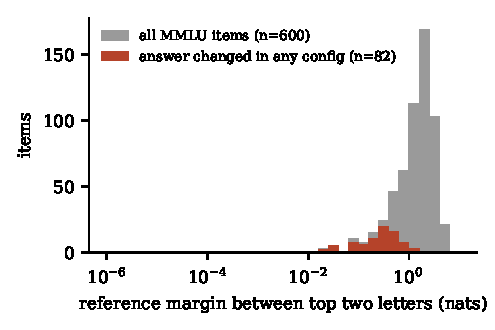
\includegraphics[width=0.49\linewidth]{fig/margins.pdf}\hfill
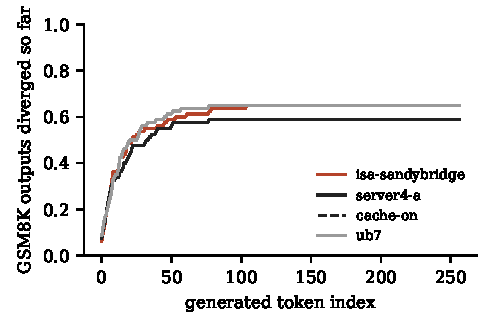
\includegraphics[width=0.49\linewidth]{fig/divergence.pdf}
\caption{Left: reference answer margins (log-probability gap between the two best letters) for
all MMLU items and for the items whose answer changed under at least one setting
(Q4\_K\_M). Changed answers come from the low-margin tail. Right: fraction of GSM8K outputs that
have diverged from the reference by each generated token index, per setting. The prompt-cache curve lies at zero.}
\label{fig:margins}
\end{figure}

\subsection{Run-to-run variation under a parallel server}
The \texttt{server4} setting is how a parallel evaluation harness usually drives
\texttt{llama-server}. Its numbers depend on request timing: how many requests share a decode
step and how prompts split across micro-batches change from run to run. For Q4\_K\_M, each of the
two runs agreed bitwise with $R$ on fewer than 12\% of items, and the two runs agreed with each
other bitwise on 45.4\% (445 of 980). They gave the same visible output on 87.9\% of items, and
33 of 80 GSM8K chains; 17 items flipped between the two runs and GSM8K accuracy happened to
match. A user who runs this command twice and compares answers sees two different models.

For the other files the parallel server mattered less, again following the format: Qwen3 Q4\_0
kept 71.6\% of items bitwise identical to $R$ and Q8\_0 73.5\%, with 6 and 3 flips. GEMMASERVER

\subsection{How large is this relative to a quantization comparison?}
To judge whether these numbers matter, Table~\ref{tab:quant} compares the four Qwen3-0.6B
formats with each other, all at $R$. Going from F16 to Q8\_0 changes 32 MMLU answers and 40 items
flip; going from F16 to Q4\_K\_M changes 173 answers and costs 8.7 MMLU points. The AVX tier change
on the Q4\_K\_M file, with no change to the weights, changed 41 MMLU answers, more than the whole
F16-to-Q8\_0 quantization step did. In teacher-forced terms the tier change on Q8\_0 (mean KLD
0.0013) is about 60\% of the divergence between Q8\_0 and F16 (0.0023), 11\% of the Q4\_K\_M-to-F16
divergence and 1.3\% of the Q4\_0-to-F16 divergence (\texttt{quantkl.py}).

So execution noise does not hide large quantization losses: the 8-point drop from F16 to
Q4\_K\_M is far outside the accuracy spread of any execution change here. It does make small
comparisons unreliable. A one- or two-point difference between two formats on a benchmark of a
few hundred items is within what a change of backend tier or server setting produces on one
file, and an answer-level comparison (which items each format gets right) is dominated by
execution noise for the closest pairs.

\begin{table}[t]
\centering\small
\caption{Differences between quantization formats of the same model, all run at $R$.
Compare with the execution-only differences in Table~\ref{tab:evalfull}.}
\label{tab:quant}
\begin{tabular}{lrrrrr}
\toprule
pair (both at $R$) & same out \% & MMLU ans. changed & flips & $\Delta$MMLU & $\Delta$GSM\\
\midrule
q06-q4km vs q06-q80 & 44.8 & 158 & 147 & +8.2 & +20.0\\
q06-q40 vs q06-q4km & 26.0 & 121 & 123 & -0.2 & -7.5\\
q06-q40 vs q06-q80 & 32.4 & 184 & 166 & +8.0 & +12.5\\
q06-f16 vs q06-q4km & 44.0 & 173 & 161 & -8.7 & -18.8\\
q06-f16 vs q06-q40 & 31.7 & 204 & 186 & -8.5 & -11.2\\
q06-f16 vs q06-q80 & 87.7 & 32 & 40 & -0.5 & +1.3\\
\bottomrule
\end{tabular}

\end{table}
